%% Version: August 28, 2011

%% Template file for Edited Books submitted to MIT Press

\documentclass{MITPress}
\usepackage{graphicx}

%% Bibliography style %%%%%%%%%%%

%% For Chicago style bibliography style, uncomment:

 \usepackage{natbib}
 \bibliographystyle{chicago}

%% To use APA style bibliography, comment out above
%% and uncomment this:

%% \usepackage[nosectionbib]{apacite}
%% \bibliographystyle{apacite}

%% Index %%%%%%%%%%%%%%%%%%%%%%%%

%% Uncomment to make index:
\usepackage{makeidx}
\makeindex

%%%%%%%%%%%%%%

%%%%%%%%%%%%%%%%%%%%%%%%%%%%%%%%%
%%% Set up Before Text Starts %%%

%% book title:
\title{}

%% possible subtitle:
\subtitle{}

%% name of author or authors
\bookauthor{}


\dedication{

% (multiple dedications possible)

% (This space may instead be used for an epigraph)
}

%% if appropriate, put Compositor name and address here:
\compositor{}

%% Series Page

\seriespage{

% for example:
%{\bf The MIT Press Free Software Series}
%
%\title{First Book}
%\author{author or authors}

% etc

}

%% if you want your sections to be numbered, uncomment
%\setcounter{secnumdepth}{3}

%%% End Set Up                %%%
%%%%%%%%%%%%%%%%%%%%%%%%%%%%%%%%%


\begin{document}

%% Title pages and Contents will not print unless this command is used:

\titlepages 


\begin{foreword}

%% foreword author:
\author{}

%% text

\authoraddress{
author name\\
address\\
date\\
}

%(Foreword should be written by someone other than author of book)

\end{foreword}

%% Optional series foreword:
%\begin{seriesforeword}

%% Author of Series Foreword
%\author{}

%Introduction to this book as part of a series, if appropriate.

% \authoraddress{
% Author of Series Foreword\\
% Address\\
% Current Date\\
% }

%\end{seriesforeword}

%%%
% Optional preface
% The preface should only be written by the author of the book.

% \begin{preface}

% \authoraddress{
% Author of Book\\
% Address\\
% Current Date\\
% }
% \end{preface}


%% Acknowledgments can optionally be included in preface, instead of
being in their own section.

% \begin{acknowledgment}

% \authorinitials{}

% \end{acknowledgment}

%% Optional introduction. Introduction could also be first chapter.

%\begin{introduction}
%\authors{}

%% Use \endnotes to make footnotes print at end of introduction or chapter
%\endnotes

%\end{introduction}




\part{}

%% version of title in square brackets goes to table of contents

%\chapter[(optional version to go to table of contents)]
%{Title to be printed}


% You are advised only to use these three levels of section heads:
%\section{}
%\subsection{}
%\subsubsection{}

%% \callout{} shows where this figure should appear. 
%% (Figures and Tables must be sent to end of chapter)
%% for instance:
%% \callout{Table 1.1}

%% Optional: instead of endnotes, use \note for short comment

%% \note
%% text...

%% For single endnote use \note and \endnote{<num>}{<text>}
%% \note
%% \endnote{1}{See the COTS-Based Systems (CBS) Iniative Web site
%% at http://www.sei.cmu.eud/cbs.}

%% Use this before figures and tables:
% \newpage

%% name your figure files with figure_(chapter)_(figure number)

%% Example figure:
%% \begin{figure}
%% 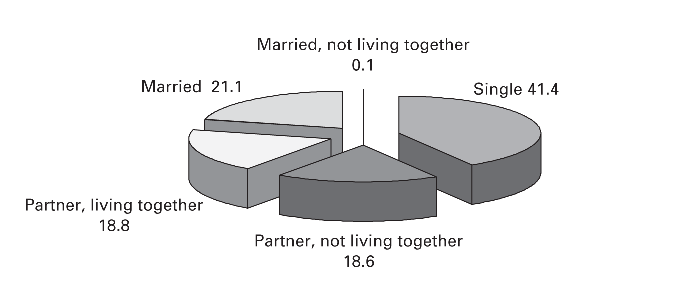
\includegraphics[width=.7\textwidth]{figure_01_01}
%% \caption{GNOME is composed of a collection of
%% libraries and applications. The libraries are
%% responsible for interacting between the user and X11 or the operating
%% system.} 
%% \end{figure}

%% \begin{table}
%% \caption{General characteristics of survey respondents}
%% \begin{tabular}{p{2in}lllll}
%% \hline
%% column headers\\
%% \hline
%% body of table
%% \hline
%% \end{tabular}
%% \end{table}

%\chapter{}

%% Optional epigram
%% \epigram{<text>}{<author>}

%%\begin{quote}...\end{quote} for short quote, one paragraph:

%%\begin{quotation}...\end{quotation} for long quote, more than one paragraph

%% Indexing:
% Comprehensive information on making an index in \LaTeX:
% http://en.wikibooks.org/wiki/LaTeX/Indexing
% part of the general \LaTeX\ reference:\\
% http://en.wikibooks.org/wiki/LaTeX

% For information on what terms to include in your index, please see:\\
% http://mitpress.mit.edu/authors/guidelines/indexing.asp

%%% End Matter %%%%


%% Optional Epilogue
% \begin{epilogue}
% \title{Epilogue: <title>}
% \author{}
% <text here>
%\end{epilogue}

%% Appendix:
% \appendix
% \chapter{}
% \author{}
% Appendix text here.



%%%%%%%%%%%%%%%%%%%%%%%%%%%%%%%%%%%%%%%%%%%%%%%%%%%%%%%%%%%%%
%%% References

%%% If, instead of using BibTeX, you want to enter your own bib entries, 
%%% follow this form, giving the author-year in the optional square
%%% bracket after \bibitem. This will make the cite produce the
%%% correct author date form: \cite{rowe} will produce (Rowe, 2011).
%%% Please use italics for book titles.

%%
% \begin{thebibliography}{Nahas, 1999} %% put widest term here to determine
                                       %% width of bibliography margin.
%bookcd
% \bibitem[Rowe, 2011]{rowe}
% Rowe, Robert. 2001. Machine Musicianship. Cambridge, Mass.: MIT Press.

%Chapter in a Book
% \bibitem[Marx, 1988]{marx}
% Marx, Leo. 1988. ``The railroad-in-the landscape: An iconological reading 
% of a
% theme in American art.'' In {\it The railroad in American art: Representations of
% technological change}, ed. Susan Danly and Leo Marx, 170--196. Cambridge,
% Mass.: MIT Press.

%Article in a Journal
% \bibitem[Nahas, 1999]{nahas}
% Nahas, Ronald C. 1999. ``Beirut rising.'' Urban Land 58 (10) (October):
% 40--46. 
% \end{thebibliography}
%%%%%%%%%%%%%%%%%%%%%%%%%%%%%%%%%%


%%%%% Bibliography using bibtex. 

% \bibliography{<filename.bib>} will
% access filename.bib for bibliography database. After you run LaTeX
% on your filename.tex file once, you can run bibtex on filename,
% then run LaTeX on filename twice to make the bibliography, and to
% update the citations.

%\bibliography{sample}

%%%%% List of Contributors
%\listofcontributors

% \section{About the Editors}

%\name{name} description
%\name{name} description
%\name{name} description

%\section{About the Contributors}

%\name{name} description
%\name{name} description
%\name{name} description

%%%%%%%%%%%%%%%%%%%%%%%%%%
%%% Index will appear here 

%% Index steps: 
%% 1. Before \begin{document}:
%%    \usepackage{makeidx}
%%    \makeindex

%% 2. Enter \index{term} or \index{term!subterm} \index{term!subterm!subterm}
%%    (no spaces before or after the !)

%% 3. Run LaTeX, producing filename .idx

%% 4. Then on command line type `makeindx filename' which will
%%     produce filename.ind. You can edit this file if you want to change
%%     anything in it.

%% 5. Now, index will appear where you type this command:

% \printindex

\end{document}
